
%\usepackage{sectsty}
\usepackage{titlesec}
\usepackage{url}

\usepackage{amssymb}

\usepackage{titlesec}

\usepackage{transparent}

\usepackage{setspace}
%\doublespacing
%\onehalfspacing

\usepackage{graphicx}
%\graphicspath{ {/ext_root/openshift-oc3/mmui-caf-local/web/mmui/public/pics/} }

\newcommand{\sectionGraphics}{

\vspace{2em}\centerline{\includegraphics[scale=0.125]{logo-deco.png}}\vspace{-1em}}

\usepackage[flushmargin]{footmisc}

\setlength{\parindent}{30pt}

%\usepackage{bigfoot}

%\DeclareNewFootnote[para]{R}[Roman]
%\DeclareNewFootnote[para]{N}

%\usepackage[letterpaper, left=1.3in,right=1in,top=1in,bottom=1in]{geometry}

\newcommand{\descItem}[1]{\item[{\color{logoRed!80!logoBlue}{\fontfamily{phv}%
\fontshape{it}\fontseries{b}\selectfont\scriptsize #1}}]}
%\newcommand{\descItem}[1]{\item[#1]}

\newcommand{\descItemLarge}[1]{\item[{\color{logoRed!80!logoBlue}{\fontfamily{phv}%
\fontshape{it}\fontseries{b}\selectfont\small #1}}]}


\usepackage{enumitem}

\setlist[description]{%
  topsep=30pt,               % space before start / after end of list
  itemsep=5pt,               % space between items
  font={\bfseries\sffamily}, % set the label font
%  font={\bfseries\sffamily\color{red}}, % if colour is needed
}


\usepackage{etoolbox}

\usepackage{mathptmx}
%\usepackage{euler}
%\usepackage{amsmath}

%\usepackage[LGRgreek]{mathastext}

%\sectionfont{\fontsize{12}{15}\selectfont}
%\subsectionfont{\fontsize{11}{12}\selectfont}

\titleformat*{\subsection}{\small\bfseries}

\usepackage{eufrak}
\usepackage{wasysym}
\usepackage{textcomp}
\usepackage{amssymb}

\usepackage{microtype}


\usepackage{graphicx}

\usepackage{tikz}

\usetikzlibrary{decorations.pathmorphing}
\usetikzlibrary{positioning}
\usetikzlibrary{shapes,snakes}


\let\OldSection\section

\renewcommand\section[1]{
	\vspace{9pt}
	
	\scalebox{1.3}{\colorbox{logoPurple!50}{\hspace{1em}}}
				
	%\hspace{-1.1cm}{\protect
\includegraphics[width=1cm]{e-logo.png}}	
	{\protect\transparent{0.3}{\colorbox{logoPeach!10!blue}{%
			\begin{minipage}{\linewidth}
				    \vspace{.5em}
				
	\protect\transparent{1}{\OldSection{#1%
		%{\transparent{0.5}{
		%	\protect
\includegraphics[width=1cm]{e-logo.png}
		%}
	    %}
     }}
	    \end{minipage}}} }
    
    \vspace{-5em}
    	{\protect\transparent{0.3}{\colorbox{logoPeach}{%
    		\begin{minipage}{\linewidth}
    			\hspace{\linewidth}
    	\end{minipage}}} } 
    
    \vspace{5em}
    
	\vspace{-6pt}
}

%\subsectionfont{\Large}
%\subsectionfont{\fontsize{12}{15}\selectfont}

\titleformat*{\subsection}{\Large\bfseries}

\renewcommand{\thesubsection}{\arabic{subsection}}

\let\OldSubsection\subsection
\renewcommand\subsection[1]{

	\vspace{-1pt}
	
    %{\LARGE
	%\colorbox{logoCyan}{%
	%\begin{minipage}{\linewidth}
		\OldSubsection{% 	
			\hspace{-2.75em}
			%\begin{minipage}{}
			\protect\raisebox{-5pt}{%
			\colorbox{logoCyan!50}{\hspace{2.1em}}}%
			\hspace{-5pt}{\protect\transparent{0.3}{\colorbox{logoBlue!80}{\protect\transparent{1}{%
						   \protect\raisebox{1pt}{\textit{{\large #1}}} }}}}
			%\end{minipage}
		}
	%\end{minipage}
    %}
    %}
	\vspace{-1pt}
}



\newcommand*{\MyCircle}{\begin{tikzpicture}{baseline}
	\node [draw, shape=regular polygon, regular polygon sides = 5, shape border rotate=180,
	line width=.2mm, left color=blGreen, right color=darkBlGreen, draw=darkRed, aspect=1,
	draw opacity=0.6, fill opacity=0.8, xscale=0.5, yscale=0.5,
	minimum width=1mm, 
	] 
	at (0, 0) {};
	\end{tikzpicture}}


\newcommand*{\MyLabel}{%
 %\MyBall	
 %{\tikz \draw [baseline, ball color=red, draw=red] circle (3pt);} 	
 \protect\MyCircle{\hspace{4pt}}\color{flColor}\LARGE{\textbf{\protect\raisebox{-3pt}{\theenumi}}}
}

%
\newenvironment{colorDescription}{%
\vspace{1em}\begin{description}[style=nextline]}{\end{description}}

\newcommand*{\MyDiamond}{%
	\begin{tikzpicture}{baseline}
	
	\node [draw, shape=diamond, %shape border rotate=100,
	line width=.2mm, left color=flColor, right color=darkRed, draw=logoPurple, aspect=1,
	draw opacity=0.6, fill opacity=0.8, xscale=0.5, yscale=0.5,
	minimum width=1mm, 
	] 
	at (2, 0) {};
	
	\end{tikzpicture}
	
} 

\usepackage{enumitem}

\newcommand*{\MyDiamon}{*} 


\newenvironment{colorItemize}{\vspace{1em}\begin{itemize}[label={\MyDiamond}]}{\end{itemize}}

\newenvironment{colorEnumerate}{\vspace{1em}\begin{enumerate}[label=\MyLabel]}{\end{enumerate}}

\newcommand{\PeoplesVoiceCafe}{{\relscale{0.8}{\fontfamily{fvs}\fontseries{b}\selectfont%
 Peoples' Voice Cafe}}}
 
\newcommand{\q}[1]{{\fontfamily{qcr}\selectfont ``}#1{\fontfamily{qcr}\selectfont ''}} 

\usepackage{tcolorbox}

%\usepackage[framemethod=TikZ]{mdframed}

%
\tcbuselibrary{skins}
%\tcbuselibrary{listings,breakable}
\usetikzlibrary{calc}
\usetikzlibrary{shadows}
\pgfdeclarelayer{background}
\pgfdeclarelayer{foreground}
\pgfsetlayers{background,main,foreground}

\definecolor{BaseColor}{HTML}{8533FF}

\newlength{\boxShadowOfset}
\setlength{\boxShadowOfset}{2mm}

\newcommand{\tc}[1]{
\vspace*{-2.05cm}\hspace{1cm}
\begin{tcolorbox}
[colframe=cyan!10!black,boxrule=0.5pt,arc=8pt,hbox,enhanced, 
leftrule=5pt,rightrule=3pt,toprule=0pt,toprule=0pt,
%drop fuzzy shadow southeast={BaseColor!50!white},
%frame code={
%        },
     % left=6pt,right=6pt,top=6pt,bottom=6pt,
      boxsep=0pt]      
\protect{#1}
\end{tcolorbox}      
\vspace*{0.4cm}

}

\newcommand{\cursive}[2]{{\LARGE%
%\begin{minipage}{0.5\textwidth}
\protect\tc{%
%\protect\fcolorbox{cyan!10!black}{white}{
\protect\raisebox{-2pt}{
{\color{logoBlue!90!cyan}{%
{\fontfamily{bch}\fontseries{b}\selectfont%
 \larger{#1}}}}}{{\color{logoBlue!90!cyan}{\Fontlukas\bfseries\textsc{#2}}}}%
%\end{minipage}
%}
}}}
%\end{minipage}

\newcommand{\parlead}[1]{\vspace{1.15em}\noindent{%
{\color{logoRed!80!logoBlue}{\fontfamily{bch}\fontseries{b}\selectfont\large #1}}}}

\newcommand{\itemLarger}[1]{\item {\raisebox{-2pt}{\larger{#1}}}}

\newcommand{\itemLargerLine}[2]{\item {\raisebox{-2pt}{\larger{#1}}}%
\hspace{1em}{\raisebox{-2pt}{#2}}}

\newcommand{\p}{

\vspace{.85em}}

\newcommand{\txtbl}{\hspace{2pt}{{\raisebox{1pt}{\relsize{-2}\textbullet}}}\hspace{2pt}}

\newcommand{\colorhref}[1]{\colorbox{blGreen!20}{#1}}



\PassOptionsToPackage{svgnames}{xcolor}

\usepackage[object=vectorian]{pgfornament} %%  http://altermundus.com/pages/tkz/ornament/index.html
\usepackage{lipsum,tikz}

\newcommand{\sectionline}[1]{%
  \noindent
  \begin{center}
  {\color{#1}
    \resizebox{0.5\linewidth}{1ex}
    {{%
    {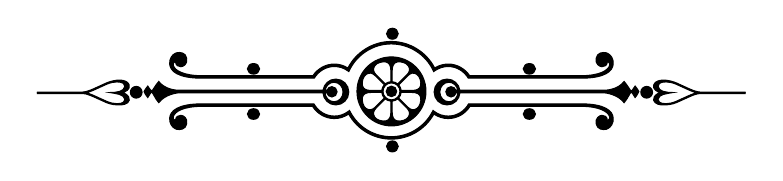
\begin{tikzpicture}
    \node  (C) at (0,0) {};
    \node (D) at (9,0) {};
    \path (C) to [ornament=84] (D);
    \end{tikzpicture}}}}}%
    \end{center}
  }
%% A macro with two arguments to change ornaments and colors easily
%% Syntax -- \sectionlinetwo{<color>}{<ornament>}
\newcommand{\sectionlinetwo}[2]{%
  \nointerlineskip \vspace{.5\baselineskip}\hspace{\fill}
  {\color{#1}
    \resizebox{0.5\linewidth}{2ex}
    {{%
    {\begin{tikzpicture}
    \node  (C) at (0,0) {};
    \node (D) at (9,0) {};
    \path (C) to [ornament=#2] (D);
    \end{tikzpicture}}}}}%
    \hspace{\fill}
    \par\nointerlineskip \vspace{.5\baselineskip}
  }

\newcommand{\EnglischeLinie}{
\sectionline{darkRed!60!cyan}
}

\newcommand{\RO}{\mbox{RO}}

\newcommand{\llMOSAIC}{\mbox{{\LARGE MOSAIC}}}
\newcommand{\lMOSAIC}{\mbox{MOSAIC}}
\newcommand{\lfMOSAIC}{\mbox{M\small{OSAIC}}}
\newcommand{\MOSAIC}{\mbox{\small{MOSAIC}}}
\newcommand{\RAK}{\mbox{\small{RAK}}}
\newcommand{\SDK}{\mbox{\small{SDK}}}
\newcommand{\lSDK}{\mbox{SDK}}
\newcommand{\GUI}{\mbox{\small{GUI}}}
\newcommand{\lfGUI}{\mbox{G\small{UI}}}
\newcommand{\qvspace}{\vspace{.4em}}

\newcommand{\textqt}[1]{{{\fontfamily{qhv}\selectfont \small{#1}}}}

\newcommand{\VersatileUX}{{\color{red!85!black}\Fontauri Versatile}%
{{\fontfamily{qhv}\selectfont\smaller UX}}}

\newcommand{\NDPCloud}{{\color{red!15!black}%
{\fontfamily{qhv}\selectfont {\smaller NDP C{\smaller LOUD}}}}}
